\documentclass[11pt,a4paper]{article}
\usepackage[utf8]{inputenc}
\usepackage[vietnamese]{babel}
\usepackage{amsmath,amssymb}
\usepackage[version=4]{mhchem}
\usepackage{geometry}
\geometry{top=1.5cm,bottom=1.2cm,left=1.4cm,right=1.4cm,headheight=28pt,headsep=12pt,footskip=18pt}
\usepackage{graphicx}
\usepackage{xcolor}
\usepackage{tabularx}
\usepackage{array}
\usepackage{tikz}
\usepackage{multicol}
\usepackage{fancyhdr}
\usepackage{enumitem}

\definecolor{hfRed}{HTML}{D32F2F}
\definecolor{hfGreen}{HTML}{8BC390}
\definecolor{mainGreen}{HTML}{2E7D32}

\usepackage{ex_test}

\pagestyle{fancy}
\fancyhf{}
\renewcommand{\headrulewidth}{0.75pt}
\renewcommand{\headrule}{\hbox to\headwidth{\color{hfGreen}\leaders\hrule height \headrulewidth\hfill}}
\renewcommand{\footrulewidth}{0.75pt}
\renewcommand{\footrule}{\hbox to\headwidth{\color{hfGreen}\leaders\hrule height \footrulewidth\hfill}}

\fancyhead[L]{\small\itshape\color{hfRed}Tài liệu lưu hành nội bộ}
\fancyhead[R]{\small\color{hfRed}Thầy \textbf{TRẦN VĂN THẠNH} - 0777.470.803}

\fancyfoot[L]{\footnotesize\itshape\color{hfRed}CS1: 6/15 Nguyễn Hoàng, P. Kim Long, TP Huế \quad|\quad CS2: 24 Đặng Thái Thân, TP Huế}
\fancyfoot[R]{\small\textbf{\color{hfRed}Trang \thepage}}

\setlength{\parindent}{0pt}
\setlength{\parskip}{1.8pt}

\def\loigiai#1{}

\begin{document}

\Opensolutionfile{ans}[ans-de11-hs]

\noindent
\begin{minipage}[t]{0.48\textwidth}
	\centering
	\textbf{SỞ GIÁO DỤC VÀ ĐÀO TẠO THỪA THIÊN HUẾ}\\
	\textbf{TRƯỜNG THPT HAI BÀ TRƯNG}\\
	\textbf{ĐỀ CHÍNH THỨC}\\
	\textit{(Đề thi có 04 trang)}
\end{minipage}\hfill
\begin{minipage}[t]{0.48\textwidth}
	\centering
	\textbf{\color{mainGreen}ĐỀ KIỂM TRA ĐỊNH KỲ CHƯƠNG 4 (POLYMER)}\\
	\textbf{MÔN: HOÁ HỌC -- LỚP 12}\\
	\textit{Thời gian làm bài: 50 phút (không kể thời gian phát đề)}\\
	\textbf{Mã đề thi: 111}
\end{minipage}


\vspace{0.1cm}
\noindent\textit{Họ, tên thí sinh: \dots\dots\dots\dots\dots\dots\dots\dots\dots\dots\dots\dots\dots\dots\dots\dots\dots\dots\dots\dots\dots\dots Lớp: \dots\dots\dots\dots SBD: \dots\dots\dots\dots}\\
\noindent\textit{(Cho biết nguyên tử khối: H = 1; C = 12; N = 14; O = 16; Na = 23; Al = 27; S = 32; Cl = 35,5; K = 39; Ca = 40; Fe = 56; Cu = 64; Zn = 65; Br = 80; Ag = 108; Ba = 137).}

\vspace{0.15cm}
\noindent
\textbf{PHẦN I (4,5 điểm -- 18 câu): Câu trắc nghiệm nhiều phương án lựa chọn.}\\
\textit{Thí sinh trả lời từ câu 1 đến câu 18. Mỗi câu hỏi thí sinh chỉ chọn một phương án.}

\setcounter{ex}{0}

\begin{ex}
(SBT -- KNTT). Chất nào dưới đây thuộc loại polymer?
\choice
{Glucose}
{Fructose}
{Saccharose}
{Cellulose}
\loigiai{}
\end{ex}

\begin{ex}
(SBT -- KNTT). Tính chất vật lí chung của polymer là
\choice
{chất lỏng, không màu, không tan trong nước}
{chất lỏng, không màu, tan tốt trong nước}
{chất rắn, không bay hơi, dễ tan trong nước}
{chất rắn, không bay hơi, không tan trong nước}
\loigiai{}
\end{ex}

\begin{ex}
Polymer nào sau đây bị thủy phân trong dung dịch \ce{NaOH}?
\choice
{Poly(vinyl acetate)}
{Polyethylene}
{Polypropylene}
{Polybuta-1,3-diene}
\loigiai{}
\end{ex}

\begin{ex}
Polymer nào sau đây có thể bị thuỷ phân hoàn toàn trong môi trường acid hoặc môi trường base thu được amino acid?
\choice
{Tinh bột}
{Tơ capron}
{Polypropylene}
{Poly(vinyl chloride)}
\loigiai{}
\end{ex}

\begin{ex}
(SBT -- KNTT). Trên hộp xốp cách nhiệt, hộp đựng thức ăn mang về, cốc, chén đĩa dùng một lần,\dots{} thường được in kí hiệu như hình bên. Polymer dùng làm các đồ dùng đó được tổng hợp từ monomer nào sau đây?
\begin{center}
	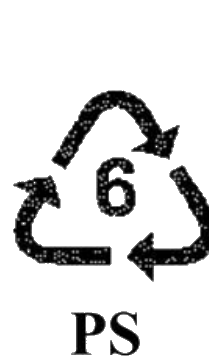
\includegraphics[width=1.5cm]{images_crop_de11/cau5_ps_symbol.png}
\end{center}
\choice
{\ce{CH2=CH2}}
{\ce{CH2=CH-CH3}}
{\ce{CH2=CH-C6H5}}
{\ce{CH2=CHCl}}
\loigiai{}
\end{ex}

\begin{ex}
(SBT -- KNTT). Phân tử polymer nào sau đây chỉ chứa hai loại nguyên tố?
\choice
{Poly(methyl methacrylate)}
{Poly(vinyl chloride)}
{Polyacrylonitrile}
{Polypropylene}
\loigiai{}
\end{ex}

\begin{ex}
(SBT -- KNTT). Tơ tằm, sợi bông, len thuộc loại tơ nào sau đây?
\choice
{Tơ tự nhiên}
{Tơ tổng hợp}
{Tơ bán tổng hợp}
{Tơ nhân tạo}
\loigiai{}
\end{ex}

\begin{ex}
(SBT -- KNTT). Tơ nào sau đây thuộc loại tơ bán tổng hợp?
\choice
{Tơ nylon-6,6}
{Tơ cellulose acetate}
{Tơ capron}
{Tơ tằm}
\loigiai{}
\end{ex}

\begin{ex}
(SBT -- KNTT). Polymer nào sau đây \textbf{không} thuộc loại cao su?
\choice
{Poly(methyl methacrylate)}
{Polychloroprene}
{Polyisoprene}
{Polybuta-1,3-diene}
\loigiai{}
\end{ex}

\begin{ex}
Cho các polymer: polyethylene, tơ nitron, tơ capron, nylon-6,6, tinh bột, protein, cao su isoprene và cao su buna-N. Số polymer có chứa nitrogen trong phân tử là
\choice
{5}
{6}
{7}
{4}
\loigiai{}
\end{ex}

\newpage

\begin{ex}
Cho các polymer sau: cellulose, amylose, amylopectin, poly(ethylene terephthalate), polybuta-1,3-diene, polyisoprene. Số polymer thiên nhiên là
\choice
{5}
{2}
{3}
{4}
\loigiai{}
\end{ex}

\begin{ex}
Có một số hợp chất sau: (1) ethylene, (2) vinyl chloride, (3) adipic acid, (4) phenol, (5) acrylonitrile, (6) buta-1,3-diene. Những chất nào có thể tham gia phản ứng trùng hợp?
\choice
{(1), (2), (5), (6)}
{(1), (2), (3), (4)}
{(1), (4), (5), (6)}
{(2), (3), (4), (5)}
\loigiai{}
\end{ex}

\begin{ex}
Dãy nào sau đây đều thuộc loại polymer tổng hợp?
\choice
{Tơ capron, tơ nitron, cao su buna}
{Polystyrene, tơ tằm, tơ nylon-6,6}
{Tơ cellulose acetate, cao su buna-S, tơ nylon-6}
{Tơ viscose, tơ olon, tơ nylon-7}
\loigiai{}
\end{ex}

\begin{ex}
Cho các polymer sau: polybuta-1,3-diene, poly(methyl methacrylate), polyacrylonitrile, nylon-6,6. Số polymer được điều chế bằng phản ứng trùng ngưng là
\choice
{3}
{2}
{4}
{1}
\loigiai{}
\end{ex}

\begin{ex}
Phát biểu nào sau đây sai?
\choice
{Trùng ngưng buta-1,3-diene thu được polymer dùng để sản xuất chất dẻo}
{Trùng hợp ethylene thu được polymer dùng để sản xuất chất dẻo}
{Trùng ngưng $\varepsilon$-aminocaproic acid thu được polycaproamide}
{Trùng hợp vinyl cyanide thu được polymer dùng để sản xuất tơ nitron (tơ olon)}
\loigiai{}
\end{ex}

\begin{ex}
Không nên ủi (là) quá nóng quần áo bằng nylon, len, tơ tằm vì
\choice
{len, tơ tằm, tơ nylon có các nhóm liên kết trong phân tử kém bền với nhiệt}
{len, tơ tằm, tơ nylon mềm mại}
{len, tơ tằm, tơ nylon là những sợi thấm nước}
{len, tơ tằm, tơ nylon không thể là phẳng}
\loigiai{}
\end{ex}

\begin{ex}
(SBT -- CTST). Khối lượng của một đoạn mạch nylon-6,6 là 27 346 amu và của một đoạn mạch capron (nylon-6) là 17 176 amu. Số lượng mắt xích trong đoạn mạch nylon-6,6 và capron nêu trên lần lượt là
\choice
{113 và 152}
{121 và 114}
{121 và 152}
{113 và 114}
\loigiai{}
\end{ex}

\begin{ex}
Tơ là những vật liệu polymer hình sợi dài và mảnh với độ bền nhất định. Cho các phát biểu sau về tơ:\\
(a) Mạch phân nhánh, xếp song song với nhau.\\
(b) Mềm, dai, không độc, tương đối bền với các dung môi thông thường và có khả năng nhuộm màu.\\
(c) Nguyên liệu quan trọng trong ngành luyện kim.\\
(d) Tơ tự nhiên: Là tơ có sẵn trong thiên nhiên như bông, sợi lanh, len lông cừu, tơ tằm,\dots\\
(e) Tơ tổng hợp: Là tơ được chế tạo từ polymer tổng hợp như polyamide (nylon, capron,\dots).\\
(f) Tơ bán tổng hợp: Là tơ xuất phát từ nguồn thiên nhiên nhưng được chế biến thêm bằng phương pháp hoá học (như tơ visco, tơ cellulose acetate,\dots).\\
Số phát biểu đúng là
\choice
{6}
{3}
{5}
{4}
\loigiai{}
\end{ex}

\newpage

\noindent
\textbf{PHẦN II (4,0 điểm -- 4 câu): Câu trắc nghiệm đúng sai.}\\
\textit{Thí sinh trả lời từ câu 1 đến câu 4. Trong mỗi ý a), b), c), d) ở mỗi câu, thí sinh chọn đúng hoặc sai.}

\setcounter{ex}{0}

\begin{ex}
(SBT -- KNTT). Polymer X có thể chịu được nhiệt độ lên tới 160 $^\circ\text{C}$ nên được dùng làm ống dẫn nước nóng, hộp đựng thực phẩm có thể sử dụng trong lò vi sóng,\dots{} Các vật dụng làm từ X thường được in kí hiệu như hình bên.
\begin{center}
	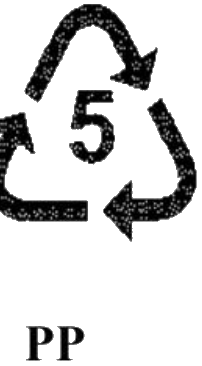
\includegraphics[width=1.5cm]{images_crop_de11/p2_cau1_pp_symbol.png}
\end{center}
\choiceTF
{X được tổng hợp từ phản ứng trùng hợp pent-1-ene}
{Hộp nhựa làm từ X có thể đựng nước sôi mà không bị biến dạng}
{X thuộc loại polymer nhiệt dẻo}
{Nhựa làm từ X thuộc loại nhựa có thể tái chế}
\loigiai{}
\end{ex}

\begin{ex}
(SBT -- CĐ). Tơ visco được sản xuất phổ biến từ đầu thế kỉ XX, là một loại chất liệu được làm từ bột gỗ của cây như tre, đậu nành, mía,\dots, qua quá trình xử lí hoá học được sợi visco. Sợi visco thấm hút mồ hôi và thoáng khí, mềm mại nên rất phổ biến trong việc sản xuất quần áo, đặc biệt là trang phục mùa hè vì nó giúp người mặc cảm thấy mát mẻ và thoải mái. Những phát biểu nào sau đây là đúng?
\choiceTF
{Tơ visco thuộc loại tơ thiên nhiên}
{Tơ visco thuộc loại tơ bán tổng hợp}
{Sợi visco có thành phần chính là cellulose đã được xử lí hoá chất}
{Tơ là vật liệu polymer hình sợi, dài, mảnh, có độ bền nhất định, mạch không nhánh}
\loigiai{}
\end{ex}

\begin{ex}
(SBT -- CĐ). Keo dán dùng để kết dính các vật liệu và được sử dụng rộng rãi trong đời sống, sản xuất. Những phát biểu nào sau đây là đúng?
\choiceTF
{Nhựa vá săm là dung dịch keo của cao su trong dung môi hữu cơ dùng để vá săm xe}
{Keo dán epoxy gồm hai thành phần là hợp chất có chứa hai nhóm epoxy ở hai đầu và chất đóng rắn}
{Bản chất của keo dán epoxy là tạo ra polymer có cấu trúc mạng không gian bền chắc, giúp gắn kết tốt hai vật liệu lại với nhau}
{Khi sử dụng keo dán poly(urea-formaldehyde) cần bổ sung chất đóng rắn để tạo polymer có mạch phân nhánh}
\loigiai{}
\end{ex}

\begin{ex}
(SBT -- KNTT). Poly(butylene adipate terephthalate) (PBAT) là một polymer có khả năng phân huỷ sinh học, có tên thương mại là Ecoflex. PBAT có đặc tính tương tự như polyethylene mật độ thấp (LDPE) nên nó được sử dụng làm túi nylon, bao bì thực phẩm phân huỷ sinh học. PBAT được điều chế từ ba monomer sau đây:
\begin{center}
	
\includegraphics[width=9.5cm]{images_crop_de11/p2_cau4_pbat_monomers.png}
\end{center}
\choiceTF
{PBAT thuộc loại polyester}
{Phản ứng tổng hợp PBAT thuộc loại phản ứng trùng hợp}
{Một mắt xích PBAT gồm 3 nhóm ester}
{Túi nylon làm từ PBAT thân thiện môi trường hơn so với LDPE}
\loigiai{}
\end{ex}

\newpage

\noindent
\textbf{PHẦN III (1,5 điểm -- 6 câu): Câu trắc nghiệm yêu cầu trả lời ngắn.}\\
\textit{Thí sinh trả lời từ câu 1 đến câu 6.}

\setcounter{ex}{0}

\begin{ex}
(SBT -- CTST). Có bao nhiêu polymer thiên nhiên trong các vật liệu sau: bông, tơ tằm, len, cellulose, tơ nitron?
\par\noindent\textit{Trả lời:} \dotfill
\loigiai{}
\end{ex}

\begin{ex}
Cho các polymer: (1) polyethylene, (2) poly(methyl methacrylate), (3) polybuta-1,3-diene, (4) polystyrene, (5) poly(vinyl acetate) và (6) tơ nylon-6,6. Trong các polymer trên, có bao nhiêu polymer có thể bị thuỷ phân trong dung dịch acid và dung dịch kiềm?
\par\noindent\textit{Trả lời:} \dotfill
\loigiai{}
\end{ex}

\begin{ex}
Một phân tử polyethylene có khối lượng phân tử bằng 56000 amu. Hệ số polymer hóa của phân tử polyethylene này là bao nhiêu?
\par\noindent\textit{Trả lời:} \dotfill
\loigiai{}
\end{ex}

\begin{ex}
Một mắt xích của polymer X gồm C, H, N. Hệ số polymer hóa của polymer này là 500 và có phân tử khối là 56500 amu. X chỉ có 1 nguyên tử N trong mỗi mắt xích. Mắt xích của polymer X có bao nhiêu nguyên tử carbon?
\par\noindent\textit{Trả lời:} \dotfill
\loigiai{}
\end{ex}

\begin{ex}
Capron là một tơ sợi tổng hợp, được điều chế từ monomer là caprolactam:
\begin{center}
	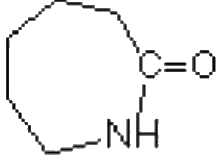
\includegraphics[width=1.5cm]{images_crop_de11/p3_cau5_caprolactam.png}
\end{center}
Một loại tơ capron có khối lượng phân tử là 14 916 amu. Số đơn vị mắt xích có trong phân tử loại tơ sợi này là bao nhiêu?
\par\noindent\textit{Trả lời:} \dotfill
\loigiai{}
\end{ex}

\begin{ex}
Polymer A trong suốt, được dùng làm hộp đựng thực phẩm, đồ chơi trẻ em, vỏ đĩa CD, DVD,\dots{} Trong công nghiệp sản xuất chất dẻo, polymer A được điều chế theo sơ đồ:
\begin{center}
	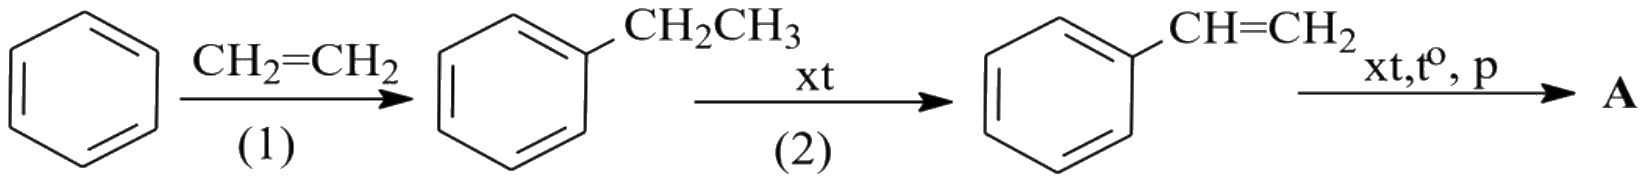
\includegraphics[width=10.5cm]{images_crop_de11/p3_cau6_scheme.png}
\end{center}
Từ $100\text{ kg}$ benzene và $32\text{ m}^3$ ethylene (ở 25 $^\circ\text{C}$, 1 bar), với hiệu suất mỗi quá trình (1), (2), (3) lần lượt là 60\%, 55\% và 60\%, hãy tính khối lượng polymer A thu được theo đơn vị kg (kết quả làm tròn đến chữ số hàng phần mười).
\par\noindent\textit{Trả lời:} \dotfill
\loigiai{}
\end{ex}


\Closesolutionfile{ans}

\end{document}
